\section{Spätná väzba užívateľov}

Testovania intuitívnosti a estetickosti užívateľského rozhrania sa účastnilo 81 osôb rôznej vekovej kategórie. Užívateľom
bolo poskytnuté zariadenie s aplikáciou a následne boli požiadaní o vyplnenie krátkeho dotazníka. Odpovede na povinné otázky
s možnosťami výberu z \textit{áno} alebo \textit{nie} sú uvedené v grafoch \ref{fig:feedbacks}.

\begin{figure}[ht!]
  \centering
  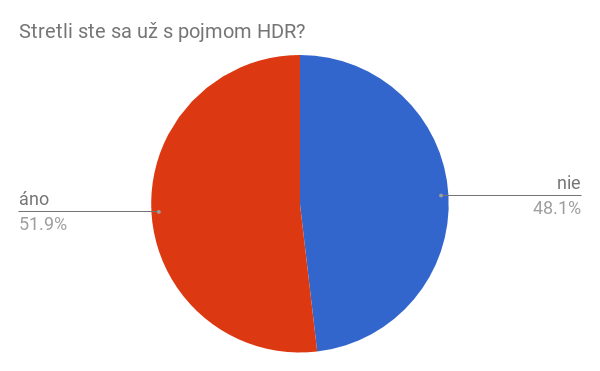
\includegraphics[width=0.45\textwidth]{figures/tests/charts/chart0}
	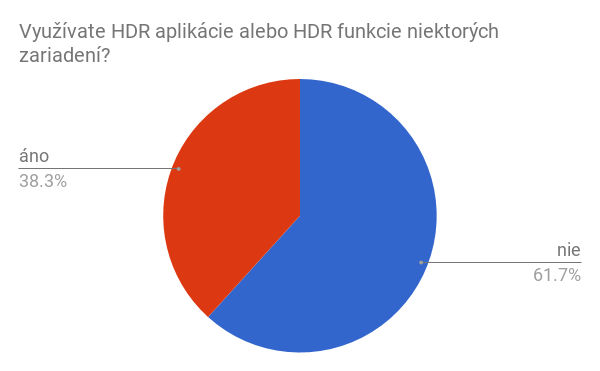
\includegraphics[width=0.45\textwidth]{figures/tests/charts/chart1}
	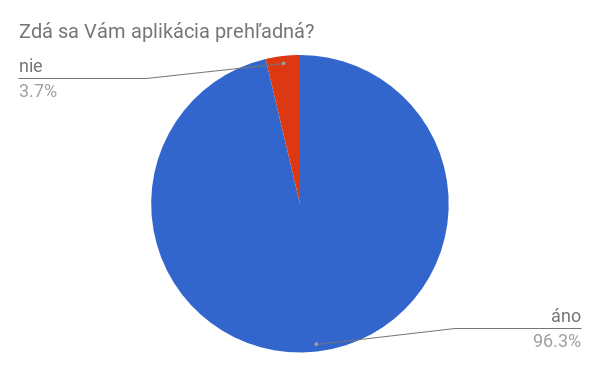
\includegraphics[width=0.45\textwidth]{figures/tests/charts/chart2}
	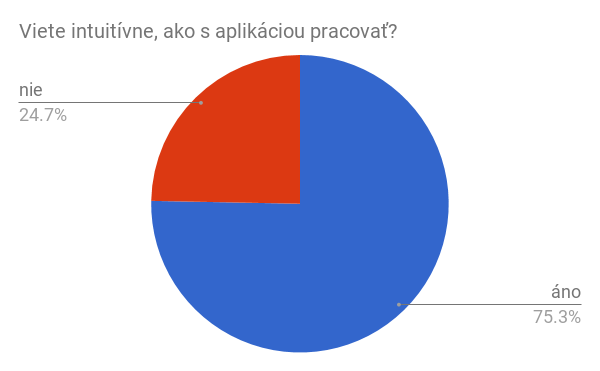
\includegraphics[width=0.45\textwidth]{figures/tests/charts/chart3}
	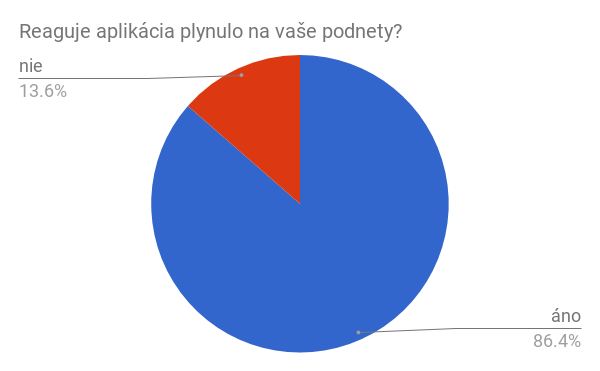
\includegraphics[width=0.45\textwidth]{figures/tests/charts/chart4}
	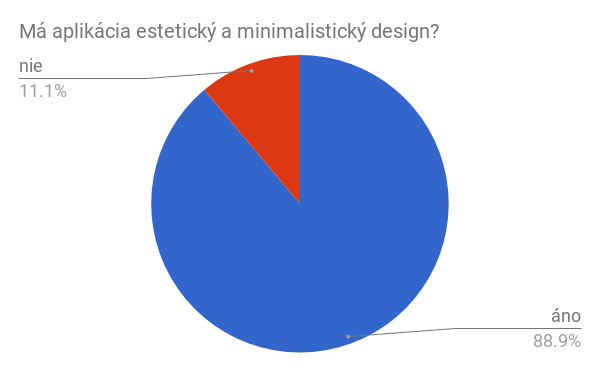
\includegraphics[width=0.45\textwidth]{figures/tests/charts/chart5}
	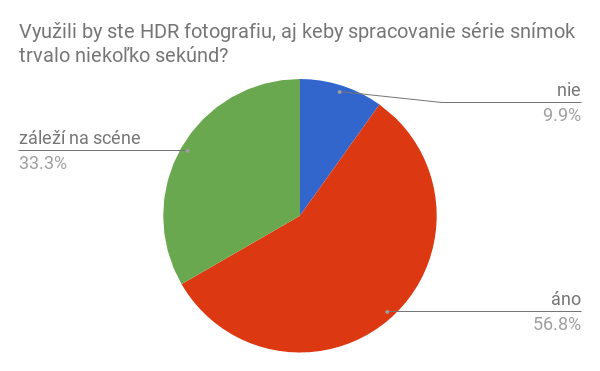
\includegraphics[width=0.45\textwidth]{figures/tests/charts/chart6}
  \caption{Odpovede testovaných užívateľov}
  \label{fig:feedbacks}
\end{figure}

Minimalistickosť aplikácie zaručuje jej prehľadnosť a ľahkú ovládateľnosť. V čase testovania užívateľov však aplikácia mala strohý,
čierno-biely dizajn a to veľa užívateľov znepokojovalo. Radi by privítali záživnejšie a farebnejšie rozhranie. Avšak vzhľadom
na ostatné aplikácie s podobným zameraním, najmä aplikácie z prieskumu existujúcich riešení, obdržal strohý, minimalistický
dizajn aplikácie pozitívne hodnotenia. Citujem odpoveď jedného respondenta:
\begin{quote}
	\textit{Aj napriek tomu, že aplikácia nesleduje najnovšie trendy mobilného dizajnu alebo pravidlá material
	designu, myslím, že je spracovaná lepšie ako veľký počet aplikácií v obchode Google Play.}
\end{quote}
Pripomienka o záživnejšie rozhranie bola zapracovaná a dnes má aplikácia príjemný modro-biely dizajn, ktorý pridáva na užívateľskom zážitku.

Najviac pripomienok mali užívatelia k tlačidlám v dolnom menu vybraného operátora. Aj napriek snahe vytvoriť ikony,
najlepšie zobrazujúce svoju funkciu, je potrebné mať v~aplikácii pomocnú obrazovku vysvetľujúcu význam jednotlivých
prvkov užívateľského rozhrania. Spracovanie tohoto požiadavku je inšpirované trendami pomocných obrazoviek mobilných aplikácií
(obrázky \ref{fig:HintScreens}). Pomocné obrazovky jednotlivých operátorov mapovania tónov dokonca obsahujú krátky popis toho,
ako daný algoritmus mapovania tónov funguje a čo znamenajú jednotlivé dôležité parametre.

\begin{figure}[ht!]
  \centering
  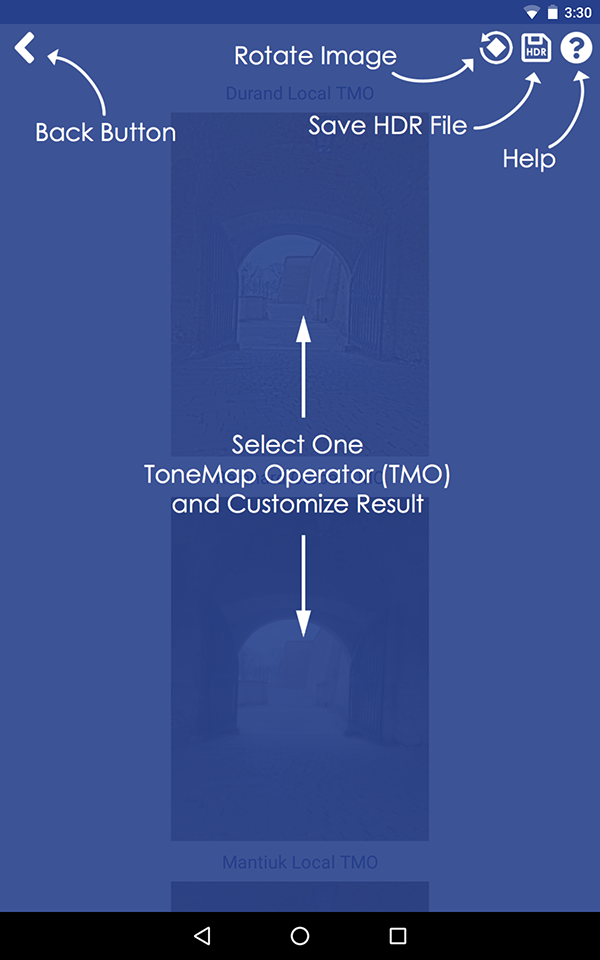
\includegraphics[width=0.35\textwidth]{figures/ui/hints/tmos}
	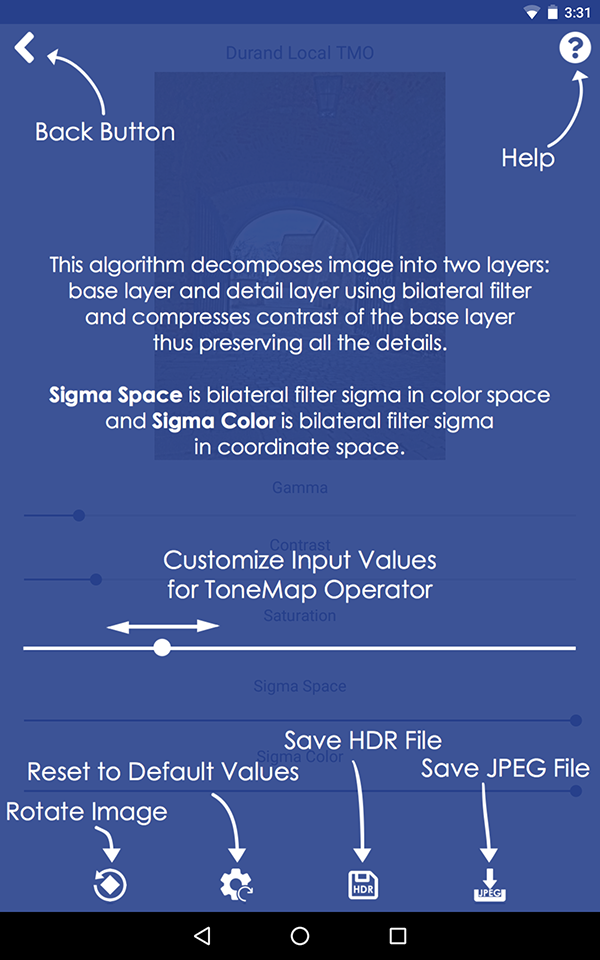
\includegraphics[width=0.35\textwidth]{figures/ui/hints/tmo}
  \caption{Vysvetlenie funkcionality jednotlivých prvkov aplikácie pomocnými obrazovkami}
  \label{fig:HintScreens}
\end{figure}

Ďalšie ohlasy boli venované tlačidlu pre zmenu orientácie obrázkov. Respondenti mali otázku, či nemôže aplikácia detekovať orientáciu
obrázku a podľa toho nastaviť východzie otočenie. Obrázky obsahujú metadáta a taktiež aj záznam o orientácii obrázku. Avšak v~tomto
prípade sa obrázok spája z viacero obrázkov a väčšina metadát sa stráca. Jednou z~možností je zapisovať metadáta ručne do súboru.
Druhá možnosť je poukázať na popredné komerčné, ale aj natívne aplikácie zariadení pre zobrazovanie obrazových súborov, ktoré obrázky
orientované na výšku tiež vo východzom nastavení neotáčajú. Neprívetivosť otáčania obrázkov je nakoniec minimalizovaná pomocou globálneho
stavu otočenia náhľadového obrázku, ktorý platí pre všetky obrazovky. Týmto sa vyhneme znovuotáčaniu náhľadového obrázku pri prechode
medzi jednotlivými operátormi a ich prehľadom. Tento stav sa resetuje pri načítaní/vytvorení nového HDR snímku.
